\chapter{Aspekte eines Anmeldesystemes und Biometrie}
\strahlhofer

%https://de.wikipedia.org/wiki/Authentifizierung
\section{Prozesse des Anmeldevorgangs}\footcite{authentifizierung}
\begin{center}
\begin{figure}[h]
    \centering
    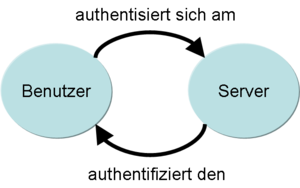
\includegraphics[width=9cm]{authentisieren-authentifizieren.png}
    \caption{Ablauf eines Anmeldevorgangs (Abbildung von Wikipedia)}
\end{figure}
\end{center}

%https://www.dr-datenschutz.de/authentisierung-authentifizierung-und-autorisierung/
\subsection{Authentisierung} 
Bei der Authentisierung muss von einer Person ein Nachweis gegeben werden, dass diese die Person ist, die sie behauptet zu sein. Dieser Nachweis kann durch drei verschiedene Methoden nachgewiesen werden. Diese sind:
\begin{itemize}
	\item Die Person besitzt Wissen über eine Information, die nur der Kontoinhaber wissen kann, zum Beispiel das Passwort oder Sicherheitsfragen.
	\item Das Individuum, das sich versucht anzumelden, sendet beispielsweise einen Reisepass oder Führerschein als Konformation.
	\item Es wird vom Nutzer eine Information mitgesendet, die er oder sie nur von sich selbst senden kann. Ein Beispiel wäre die Sendung eines biometrischen Nachweises, das kann entweder ein Fingerabdruck oder ein Gesichtsscan sein\footcite{anmeldevorgangs}.
\end{itemize}


%https://www.dr-datenschutz.de/authentisierung-authentifizierung-und-autorisierung/
\subsection{Authentifizierung}
Bei diesem Schritt des Anmeldeablaufs wird eine Überprüfung durchgeführt. Diese Prüfung analysiert die Informationen, die bei der Authentisierung erfasst worden sind. Können diese dem Zielkonto zugewiesen werden, dann ist der Nutzer die Person, die er angibt zu sein\footcite{anmeldevorgangs}.


%https://www.dr-datenschutz.de/authentisierung-authentifizierung-und-autorisierung/
\subsection{Autorisierung}
Die Autorisierung hat als Funktionalität die Bestätigung von bestimmten Rechten und Rollen zu bestimmten Ressourcen. Dieses Thema gehört der Informationssicherheit an und befasst sich mit der Zugriffskontrolle. Bei der Autorisierung wird für das Unternehmen ein Zugriffsmechanismus implementiert. Wenn zum Beispiel ein Promoter in einem von der Firma erstellten System anmeldet, werden bestimmte Rollen und Rechte zugewiesen. Dies bedeutet das der Mitarbeiter nur einen bestimmten Zugriff auf gewisse Funktionalität besitzt\footcite{anmeldevorgangs}.



\section{Biometrie}
%https://en.wikipedia.org/wiki/Biometrics
\subsection{Definition}
\begin{center}
	\textit{Biometrics are body measurements and calculations related to human characteristics\footcite{biometrie}.}
\end{center}

Bei diesem Vorgang schließt eine biometrische Identifikation nur auf eine bestimmte Person und ist gleichzeitig sehr schwer zu fälschen.
Durch diesen Aspekt ist die Biometrie eine sehr angesehene Technik in der Identifikation von Menschen\footcite{biometrie}.

\subsection{Methoden der Biometrie}
Eine biometrische Information kann durch unterschiedliche Methoden erhoben werden.
\begin{itemize}
	%https://www.ibia.org/biometrics-and-identity/biometric-technologies/dna#:~:text=DNA%20Biometrics,often%20in%20forensics%20and%20healthcare.&text=A%20feature%20of%20DNA%20identification,familial%20relationships%20via%20DNA%20testing.
	\item \textbf{DNA-Tests:} Ein DNA-Test wird in den unterschiedlichsten Arbeitsbereichen verwendet, zum Beispiel in der Forensik.
	Vorteile die DNA als biometrisches Mittel zu erwägen:
	\begin{itemize}
		\item Mit der DNA kann von einer unbekannten Person auf dessen Verwandten geschloßen werden. Dies ist die einzige biometrische Methode, die diese Möglichkeit bietet.
		\item-DNA Spuren und Fingerabdrücke können bei Tatorten gefunden werden. Diese Methode hilft Ermittlern schneller die Identität einer Person herauszufinden\footcite{dna-test}.
	\end{itemize}
	%https://de.wikipedia.org/wiki/Fingerabdruck
	\item \textbf{Fingerabdruck:} Die Fingerabdrücke sind bei jedem Menschen unterschiedlich. 
	Es gibt bis zum heutigen Tag keine bewissenen Fingerabdruckstest der auf zwei verschiedene Menschen schließen konnte. 
	Nicht einmal eineiige Zwillinge besitzen den gleichen Abdruck.
	Dieser Aspekt macht diese Methode so genau. Es wird hier von einer Einzigartigkeit gesprochen.
	\paragraph{Vorteile}
	\begin{itemize}
		\item Wie schon beschrieben werden Fingerabdrücke von Ermittlern verwendet, um die Identität von Opfern oder verdächtigen Personen aufzudecken.
		\item Der Fingerabdruck wird bei den meisten Smartphones in der heutigen Zeit per eingebauten Scanner ermittelt. Diese biometrischen Informationen werden erhoben, um das Gerät einer bestimmten Person oder auch Personen zuzuordnen.
	\end{itemize}
	\paragraph{Nachteile}
	\begin{itemize}
		\item In dem Fall, dass sich eine Person auf dem Finger verletzt, kann es dazu führen, dass der Fingerabdruck sich verändert. Aus diesem Grund kann sich die Person möglicherweise nicht mehr identifizieren\footcite{fingerabdruck}.
	\end{itemize}
	%https://en.wikipedia.org/wiki/Facial_recognition_system
	%https://www.pcs.com/wissens-werte/biometrie/gesichtserkennung-von-angesicht-zu-angesicht#:~:text=Hohe%20Sicherheit%20ist%20mit%20Gesichtserkennung,in%20der%20Regel%20nicht%20erkannt.
	\item \textbf{Gesichtserkennung:} Hier wird ein Foto oder Video analysiert und überprüft ob diese Person mit den schon aufgenommenen Bildern in der Dantebank übereinstimmen. Hier werden Aspekte wie Abstand von Augen-Nase-Mund festgestellt.
	\paragraph{Vorteile}
	\begin{itemize}
		\item Eine Person hat keinen oder kaum einen Aufwand, um sich bei dieser Methode zu identifizieren. Bei Smartphones muss man lediglich in die Frontal Kamera schauen.
		\item Gesichtserkennungssysteme besitzen den Vorteil mehrere Personen aufeinmal zu erkennen. Beispielsweise in einem Labor dürfen nur bestimmte Personen zutreten. Wenn zwei Personen nun gleichzeitig eintreten wollen und einer die Berechtigung dazu nicht besitzt, wird ein Alarm ausgelöst.
	\end{itemize}
	\paragraph{Nachteile}
	\begin{itemize}
		\item Eineiige Zwillinge können bei dieser Methode schwer unterschieden werden, da diese über ein fast identisches Gesicht besitzen\footcite{gesichtserkennung-1}\footcite{gesichtserkennung-2}.
	\end{itemize}
\end{itemize}


%https://candytech.in/10-worthy-fingerprint-scanner-smartphones-in-india/#:~:text=Motorola%20was%20the%20first%20company,fingerprint%20scanner%20at%20the%20top.
%https://en.wikipedia.org/wiki/Android_(operating_system)
\subsection{Biometrie auf Android Geräten}
Android ist eine Betriebssystem für Smartphones und Tablets. Der Erfolg des Betriebssystems, zeichnet sich damit aus, dass es Open Source ist. Das bedeutet ein Unternehmen kann Android frei und ohne Kosten nutzen.
\paragraph{Fingerabdruckssensoren:}
Motorola hatte im Jahre 2011 das Motorola Atrix veröffentlicht. Dies war das erste Smartphone auf dem Weltmarkt, dass einen Fingerabdruckssensor eingebaut hatte.
Dieses Gerät bekam durch dieses Feature einen sehr hohen Bekanntheitsgrad und löste damit gleichzeitig einen Technologietrend aus.
Des Weiteren begannen dann andere Smartphone Hersteller auch diesen Sensor zu integrieren.
Über die Jahre sind viele verschiedene Arten von Sensoren entwickelt worden. Wie zum Beispiel
\begin{itemize}
	\item Berühren eines Knopfes auf dem Gerät (zum Beispiel Apple Geräte).
	\item Wischen über einen Knopf (zum Beispiel Samsung S7 Edge).
	\item In-Display, den Finger auf das Display legen (zum Beispiel Oneplus 8)\footcite{fingerabdruck-android-1}\footcite{fingerabdruck-android-2}. 
\end{itemize}
%https://www.kiroku-just-write.de/2020/09/01/gesichtserkennung/#:~:text=Die%20grunds%C3%A4tzliche%20Voraussetzung%20f%C3%BCr%20funktionierende,f%C3%BCr%20jeden%20Menschen%20einzigartig%20sind.
\paragraph{Gesichtserkennung}
Die Gesichtserkennung gibt es schon für die meisten Android Geräte. Diese sind häufig sehr unsicher, es exisitieren viel Fälle wo das Feature geknackt worden ist. Aus diesem Grund kennzeichnen die meisten Hersteller diese Methode als unsicher\footcite{gesichtserkennung-android}. 

%https://www.consumentenbond.nl/veilig-internetten/gezichtsherkenning-te-hacken
\paragraph{consumentenbond}
Im Jahre 2019 wurde eine Studie von einer niederländischen Organisation zu dem Thema Gesichtserkennung bei Smartphones durchgeführt. 
Diese haben 60 Smartphones von unterschiedlichen Herstellern getestet. 26 dieser Handys konnten mittels eines Porträts des Telefonbesitzers entsperrt werden.\footcite{consumentenbond}


%https://en.wikipedia.org/wiki/Apple_Inc.
%https://en.wikipedia.org/wiki/Touch_ID
\subsection{Biometrie auf iOS Geräten}
Apple Inc. ist ein Technologie Unternehmen aus den Vereinigten Staaten, die durch den Verkauf von Computern in den Siebziegerjahren. Das Unternehmen bringt jährlich Smartphones (iPhones), Tablets (iPads), Laptops (MacBooks) auf den weltweiten Markt\footcite{apple}.
\paragraph{Touch ID}
Nachdem im Jahre 2012 kaufte Apple das Unternehmen AuthenTec. Dieses Unternehmen spezialisierte sich auf das Lesen von Fingerabdrücken.
Im darauffolgenden Jahr brachte das Unternehmen dann das iPhone 5s heraus. Dieses Gerät hatte einen Fingerabdruckssensor im Home-Button eingebaut. Ab diesem Zeitpunkt konnten alle Benutzer zusätzlich zu ihrem Passwort eine sogenannte Touch ID zur Identifikation benutzen.
Die Fingerabdrücke wurden auf den Chips des Geräts gespeichert, anstatt in der Cloud. Das macht Angreifern es unmöglich, die biometrischen Informationen abzufangen\footcite{touchid}.

%https://www.pcwelt.de/international/Gesichtserkennung-auf-Android-Smartphones-einrichten-10824319.html
\paragraph{Face ID}
Das erste Smartphone von Apple, dass Gesichstserkennung besitzte, war das iPhone X (2017). Dieses Feature trug den Namen Face ID und löste größtenteils damit die Touch ID ab.
Alle Geräte, die Face ID verwenden, haben eine Frontalkamera mit 3-D-Sensoren die mehr Gesichtsmerkmale erkennen als wie bei Androidgeräten\footcite{faceid}.


\subsection{Biometrie bei EMS}
Bei der Plannung der Software von EMS wurde ein Framework namens Ionic, das auf Angular aufbaut, verwendet. Dieses kann ein Projekt in zwei fast identisch aussehende Applikationen umwandeln, die auf Android und iOS laufen.
In der Dokumentation wurde Fingerprint AIO vorgestellt. Dieses Tool ist eine von Cordova bereitgestelltes Plugin, um einen Fingerabdruck auf iOS und Android zu verwenden.
Dieses Feature kann auch beispielsweise mit Face ID bei iOS Geräten verwendet werden.

\paragraph{Umfrage:} Die Gruppe hatte zwei Ideen biometrische Identifikation in die Applikation zu integrieren. Ein Vorschlag war nach dem der Benutzer sich eingeloggt und SSO ausgewählt hat, kann der Fingerabdruck zur Anmeldung verwendet werden.
Eine andere Idee war vor jeder Anfrage, die gestellt wurde, die biometrischen Daten überprüft werden.

Es wurden dafür 10 verschiedene Personen im Alter von 16 bis 20 Jahren befragt. Das Resultat hatte ergeben, dass 8 von 10 Personen bei jeder Ticketanfrage einen Identifikationsprozess durchführen.
Des Weiteren wurde gefragt, ob beide Vorschläge realisiert werden sollen. Hier haben 10/10 darauf eingestimmt das nur eines dieser Vorhaben realisiert werden soll. Der Grund war zumeist, dass eine zu häufige Abfrage störrend sein kann.

\paragraph{Umsetzung:} Die Biometrie wurde jetzt so umgesetzt, dass vor einer Anfragenstellung der Fingerabdruck überprüft wird.
